\documentclass[12pt]{article}

\usepackage{graphicx,booktabs}
\usepackage{caption,subcaption,epsfig,epstopdf}
\usepackage{float}

\usepackage{pslatex,multicol,verbatim,wrapfig,pdfpages,url}

\title{Parallel Molecular Dynamics with a Time-Reversible Nos\'{e}-Hoover Thermostat on CPUs and GPUs}
%\subtitle{APC 523}

\author{Nathan Mahynski \and George A. Khoury \and Carmeline Dsilva}


\begin{document}

\maketitle

\section{Introduction}


Due to the dramatic increase in computing power over the last thirty years, molecular dynamics (MD) simulations have become a remarkably fruitful tool for scientific discovery and engineering exploration \cite{Karplus2002,Levitt2001}.
%
These simulations allow us to screen potential drug compounds \cite{Jorgensen2004}, explore protein folding dynamics \cite{Duan1998,Shaw2010,Piana2013,Lindorff-Larsen2011}, study \cite{Boero1998} and develop \cite{Zipoli2010} new catalysts, and explore extreme conditions (temperatures and pressures) that are experimentally inconvenient all without running expensive and time-consuming experiments in a laboratory.
%
Early atomistic simulations were capable of running at only short physical timescales (picoseconds \cite{Karplus1979}), but due to enhancements in algorithms, hardware, and parallelization, physically relevant timescales (milliseconds \cite{Kohlhoff2014}) can now be tractably explored on current computers.

At its core, molecular dynamics numerically integrates Newton's equation of motion ($force = mass \times acceleration$) forward in time.
%
Different numerical integration schemes result in different numerical accuracies for the simulations.
%
Standard molecular dynamics fixes the number of particles, volume, and total energy of the system.
%
However, one can introduce thermostats and barostats to the integration algorithm to adjust the temperature and pressure of the system to attempt to keep them constant (See Figure~\ref{fig:mdfigure}).

\begin{figure}
\centering
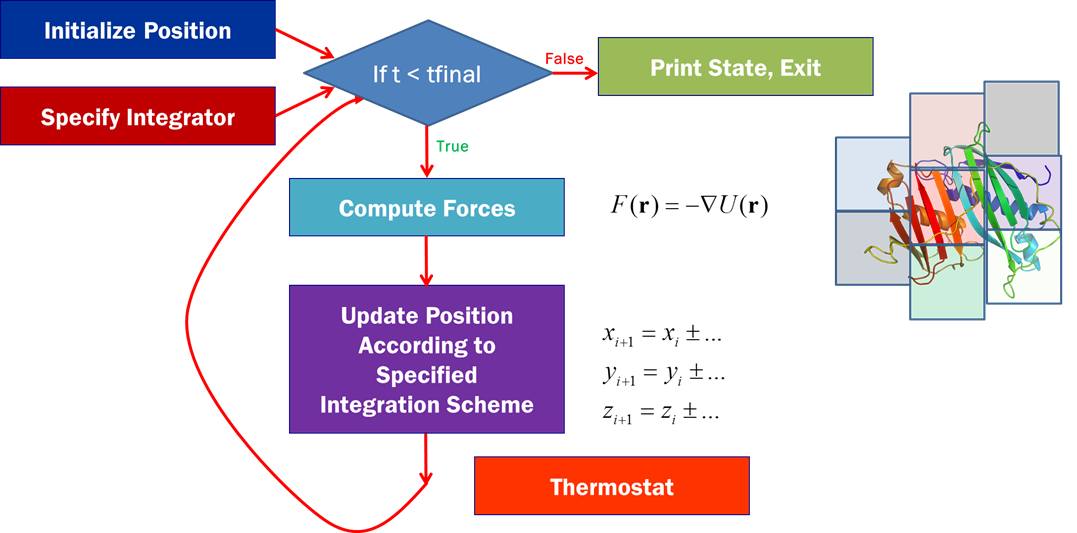
\includegraphics[width=0.65\textwidth]{mdfigure.png}
\caption{Molecular Dynamics algorithm graphical overview. MD begins with a system of particles coordinates and velocities, and integrates Newton's equation of motion forward in time utilizing a specified algorithm. A thermostat can be used to control the temperature through physics-based relationships between velocities and temperature. In this work, we implement the Nos\'{e}-Hoover Thermostat to control temperature.}
\label{fig:mdfigure}
\end{figure}

Several molecular dynamics packages exist to perform parallelized atomistic molecular dynamics simulations on CPUs.
%
These include LAMMPS \cite{Plimpton1995}, AMBER \cite{Case2010}, CHARMM \cite{MacKerell1998}, GROMACS \cite{Scott1999}, and TINKER \cite{Ponder2003}.
%
Only very recently, some of these packages have been updated in order to be implemented on Graphics Processing Units (GPUs) \cite{Brown2012,Brown2011,Gotz2012,Salomon-Ferrer2013}, and new packages exclusive to GPUs such as HOOMD-Blue\cite{Anderson2008} have been developed. %
The newly updated codes have not been nearly as extensively tested as their native CPU codebases, but can potentially offer significant speedups as pointed out by the AMBER developers (\url{http://ambermd.org/gpus/}).

Therefore, in this work we built a new software package from scratch to run molecular dynamics simulations in parallel on both CPUs and GPUs. The GPU implementation is an ambitious goal very much working on the cutting-edge of computational science since few and only recent implementations exist on GPUs \cite{Anderson2008,Brown2012,Brown2011,Gotz2012,Salomon-Ferrer2013}.
%
The GPU implementation offers the promise of a significant speedup over CPU-only implementations.
%
The software implements the Lennard-Jones potential for interatomic interactions, a velocity-Verlet integrator, and a Nos\'{e}-Hoover thermostat. The developed software is sufficiently modular that other integration algorithms and pair potentials can easily be incorporated in future versions.
%
We chose to include the Lennard-Jones potential because many of the standard force fields \cite{Case2010,MacKerell1998,Scott1999,Kaminski2001,Arnautova2006,Khoury2013} today are built on Lennard-Jones interactions.
%
For example, a commonly used model for water, the TIP3P water model \cite{Jorgensen1983}, is composed of Lennard-Jones interactions and an additional electrostatic term to account for water's ability to be polarized.
%
In addition, Lennard-Jones particles serve as a very good model for monotomic gases such as argon \cite{Rahman1964} and condensed amorphous phases such as glasses \cite{Debenedetti2001}.

Because parallelization is essential for modern day molecular dynamics software, we implemented our software to run in parallel on both CPUs (with shared memory) and GPUs.
%
Our code is therefore fairly flexible and applicable to many different hardware architectures.

\section{Theory and Algorithms}

In the following section, we describe the theory and algorithms that underly the software developed.
%
In what follows, we assume that our system of interest consists of $N$ particles.
%
We denote the position, velocity, and acceleration of particle $i$ as $\mathbf{r}_i$, $\mathbf{v}_i$, and $\mathbf{a}_i$, respectively.
%
We denote the force on particle $i$ as $\mathbf{F}_i$.

In general, the algorithm for a molecular dynamics simulation is as follows (See Figure~\ref{fig:mdfigure}):

\begin{enumerate}
\item Initialize particle positions $\mathbf{r}_i$ and velocities $\mathbf{v}_i$ within the simulation box.
\item  \label{itm:MD_start} Calculate the forces $\mathbf{F}_i$ on each particle.
\item \label{itm:MD_end} Integrate forward the positions and velocities of each particle for the chosen timestep $\Delta t$.
\item Repeat steps \ref{itm:MD_start}-\ref{itm:MD_end} for the chosen amount of simulation time.
\end{enumerate}


% Here we show overall figure.
\subsection{Integrator} \label{subsec:integrator}

We implemented a velocity-Verlet integration algorithm \cite{Swope1982}, which is accurate to fourth order.
%
For a fixed number of particles (N), volume of the system (V), and energy (E), we update the positions and velocities of each atom using the following equations
\begin{eqnarray}
\mathbf{r}_i (t + \Delta t)  & = & \mathbf{r}_i(t) + \mathbf{v}_i(t) \Delta t + \mathbf{a}_i(t) \frac{\Delta t^2}{2} \\
\mathbf{v}_i(t + \Delta t) & = & \mathbf{v}_i(t) + \left[\mathbf{a}_i(t) + \mathbf{a}_i(t + \Delta t) \right] \frac{\Delta t}{2}
\end{eqnarray}
where $\mathbf{a}_i = \mathbf{F}_i/m$.
%
The forces can be calculated from the potential energy function and will be discussed further in subsection \ref{subsec:potential}.

Because $\mathbf{v}_i$ depends on both $\mathbf{a}_i(t)$ and $\mathbf{a}_i(t+\Delta t)$, the order of computations goes as follows
\begin{enumerate}
\item Calculate $\mathbf{r}_i(t + \Delta t)$ from $\mathbf{r}_i(t)$, $\mathbf{v}_i(t)$, and $\mathbf{a}_i(t)$.
\item Calculate $\mathbf{a}_i(t + \Delta t)$ from $\mathbf{r}_i(t + \Delta t)$.
\item Calculate $\mathbf{v}_i(t + \Delta t)$ from $\mathbf{v}_i(t)$, $\mathbf{a}_i(t)$, and $\mathbf{a}_i(t + \Delta t)$.
\end{enumerate}

\subsection{Thermostats} \label{subsec:thermostat}
The equations in \ref{subsec:integrator} are only for NVE simulations.
%
If we are instead interested in fixing temperature (T) rather than energy (E), we must introduce the idea of a {\em thermostat} to our simulations.
%
A thermostat is necessary in most simulations since experiments are not typically done at constant energy.
%
The thermostat adjusts the velocities of the particles so that they (on average) maintain a user-specified desired temperature.

We implemented a time-reversible Nos\'{e}-Hoover thermostat in our molecular dynamics software.
%
The Nos\'{e}-Hoover thermostat adjusts the particle velocities based on the target temperature of the system and the current kinetic energy of the system.
%
The thermostat is governed by its own equation of motion given by the position ($\xi$), velocity ($\dot{\xi}$), and acceleration ($\ddot{\xi}$) of the thermostat.

Let $T_{set}$ be the desired temperature.
%
Then the acceleration of the thermostat is given by
\begin{equation}
\ddot{\xi} = \frac{1}{Q} \left[ \sum_{i=1}^{N} m_i v_i^2 - N_f k_B T_{set} \right]
\end{equation}

The equations of motion for the particles and the thermostat are

\small
\begin{eqnarray}
r_i(t + \Delta t) &=& r_i(t) + v_i(t) \Delta t + \left[ a_i(t) - v_i(t)\dot{\xi}(t) \right] \frac{\Delta t^2}{2}\\
v_i(t + \Delta t) &=& v_i(t) + \left[ a_i(t) - v_i(t) \dot{\xi}(t) \right] \frac{\Delta t}{2} + \left[a_i(t + \Delta t)  - v_i(t + \Delta t) \dot{\xi}(t + \Delta t) \right] \frac{\Delta t}{2} \\
\xi(t + \Delta t) & = & \xi(t) + \dot{\xi}(t) \Delta t + \ddot{\xi}(t) \frac{\Delta t^2 }{2} \\
\dot{\xi}(t + \Delta t)  & = & \dot{\xi}(t) + \left[ \ddot{\xi}(t) + \ddot{\xi} (t + \Delta t)  \right] \frac{\Delta t}{2}
\end{eqnarray}
\normalsize

The Nos\'{e}-Hoover thermostat can be shown to be time-reversible when it is implemented via the following algorithm.
First, update the thermostat velocity using a half-step in time
\begin{equation}
\dot{\xi} (t+ \Delta t/2) = \dot{\xi}(t) + \ddot{\xi}(t) \frac{\Delta t}{2}
\end{equation}
and thermostat position.
\begin{equation}
\xi (t+ \Delta t) = \xi(t) + \dot{\xi}(t+\Delta t/2)\Delta t
\end{equation}
Second, evolve the particle velocities with a half-step.
\begin{equation}
v_i (t+\Delta t/2) = v_i (t) \exp^{-\dot{\xi}(t+\Delta t/2) \Delta t/2} + a_{i} (t) \Delta t/2
\end{equation}
Third, evolve particle positions.
\begin{equation}
r_{i} (t+\Delta t) + r_{i} (t) + v_{i}(t+ \Delta t/2) \Delta t
\end{equation}
Fourth, call the function \textbf{calcForce} to update the accelerations at the next timestep.
\begin{equation}
a_{i} (t+\Delta t) = F_{i} (t+ \Delta t)/m_{i}
\end{equation}
Fifth, evolve the particle velocities.
\begin{equation}
v_{i} (t+ \Delta t)  = [v_{i}(t+\Delta t/2) + a_{i}(t+\Delta t) \Delta t/2]\exp^{-\dot{\xi}(t+\Delta t/2) \Delta t/2}
\end{equation}
Finally, the thermostat velocity is updated.
\begin{equation}
\dot{\xi}(t+\Delta t) = \dot{\xi} (t+\Delta t/2) + \ddot{\xi} (t+\Delta t) \Delta t /2
\end{equation}
The thermostat acceleration, $\ddot{\xi}(t)$ is expressed in the form
\begin{equation}
\ddot{\xi}(t) = \frac{1}{\tau^{2}} [\frac{T(t)}{T_{target}} -1 ]
\end{equation}
where $\tau^{2} = \frac{Q}{(3N-1)*T_{target}}$ and $Q$, which is the thermal mass of the thermostat spring equal to unity (although it is adjustable).
Because this algorithm is time-reversible, we implemented it in our software.
% END OF THAT DOC.

The ability for this algorithm to be time-reversible is the result of a Trotter factorization of the Liouville propagator derived by Martyna and coworkers 20 years ago. Through their Trotter factorization they proved that any resulting integrator will be time-reversible \cite{Tuckerman1992}.

\subsection{Pair potentials} \label{subsec:potential}

We implemented a shifted Lennard-Jones pair potential in our molecular dynamics software.
%
In the shifted Lennard-Jones potential, the potential energy of interaction between two particles is a function of the interatomic distance $r = \|\mathbf{r}_i - \mathbf{r}_j \|$, and is given by
\begin{equation}
U(r) = 4 \epsilon\left[ \left( \frac{\sigma}{r-\delta} \right)^{12} - \left( \frac{\sigma}{r-\delta} \right)^6 \right] + U_{shift}
\end{equation}
where $\epsilon$, $\sigma$, $\delta$, and $U_{shift}$ are adjustable parameters.
%
The total potential energy of the system is then given by
\begin{equation}
U_{tot} = \sum_{i=1}^{N} \sum_{j=1}^{i-1} U\left( \| r_i - r_j \| \right)
\end{equation}

The force on a particle $F_i$ is the negative gradient of the potential, $F_i = -\nabla_i U_{tot}$.
%
It can be shown that
\begin{equation}
F_{i, x} = -\sum_{j \ne i} \frac{d U\left( \| r_i - r_j \| \right)}{d \| r_i - r_j \| } \frac{x_i - x_j}{\|r_i - r_j\|}.
\end{equation}

The potential energy and force calculations involve at worst-case $\mathcal{O}(N^2)$ calculations, since each of the $N$ particles can interact with the remaining $N-1$ particles.
%
Therefore, the potential energy and force calculation are the portions that are typically parallelized and optimized in an MD code.

\subsection{Parallelization}

We implemented parallelization on CPUs and GPUs in our molecular dynamics software.
%
On CPUs, we parallelized our code using OpenMP and therefore, our code can run in parallel on any shared memory cluster.
%
On GPUs, we parallelized our code using CUDA.
The parallelization on GPUs is implemented in the force calculation, which accounts for 27\% percent of the cost of the simulation according to our profiling studies (see Table~\ref{tab:profiling}).
%
Parallelization and scaling were tested on the TIGER cluster, and through a private GPU cluster, ANDROS through the Panagiotopoulos Lab due to unusually heavy usage of TIGER GPUs over the past month.

\subsubsection{CUDA}
CUDA stands for Compute Unified Device Architecture and is the product of the NVIDIA corporation.  CUDA is a programming language  that extends the C and C++ languages to allow a user to perform highly accelerated Single Instruction Multiple Data (SIMD) calculations by taking control of a GPU device.  Although this is a complex topic which cannot be discussed in complete detail here, the basic principle of a
GPU code is to allocate memory on the device, copy information from the host CPU to the device into the previously allocated slot(s), perform calculations, then copy the results back.  Clearly, this process is bandwidth limited as will be discussed in detail in following sections.  To simplify the above process, a very convenient library called \textbf{thrust} has been developed which essentially extends the C++ STL onto GPU devices and takes advantage of iterators, scoping, etc. which make coding significantly easier.  This is now a standard in modern versions of CUDA (version 4.0 and greater).

CUDA code must be written in files with a ``.cu" extension to be interpreted by the nvcc compiler.  The CUDA toolkit used to compile and run the code must be the same.  On TIGER, we used the module cudatoolkit/5.5.22 which must be loaded before compilation and in the submission script for jobs.  Furthermore, the correct version flags must be enabled during compilation to make thrust work properly.  For the K20 GPUs on TIGER this requires the compiler flag ``NVFLAGS = -gencode arch=compute\_35,code=sm\_35" (see Makefile\_cuda).  The success of GPU codes is very sensitive to these details, and failure to strictly adhere to these (and many other) subtleties can produce code which compiles without error, but whose run time behavior is erroneous.

A CUDA kernel function is a function which, when invoked, performs SIMD operations on a team of threads, processed in groups called warps.  Each warp is 32 threads, and there are a set number of threads per ``block".  Each block of threads is loaded on the GPU as a single unit and has access to shared memory allowing them to communicate locally but not with threads in other blocks.  To do so, global, constant, and texture memory must be used, and are valuable resources.  You will see we have included a class called systemProps in cudaHelper.h (also see cudaHelper.cu) which evaluates the properties of each device the code detects on a CPU host such as the maximum number of threads per block, etc. allowing the code to dynamically adjust to different GPUs.  We have found that a block size of 512 threads is roughly optimal, which is set in main.cpp.  Because the GPUs are generally memory and bandwidth limited, we set out to design an algorithm that uses a minimal amount of memory when performing GPU operations.

\begin{figure}[H]
   	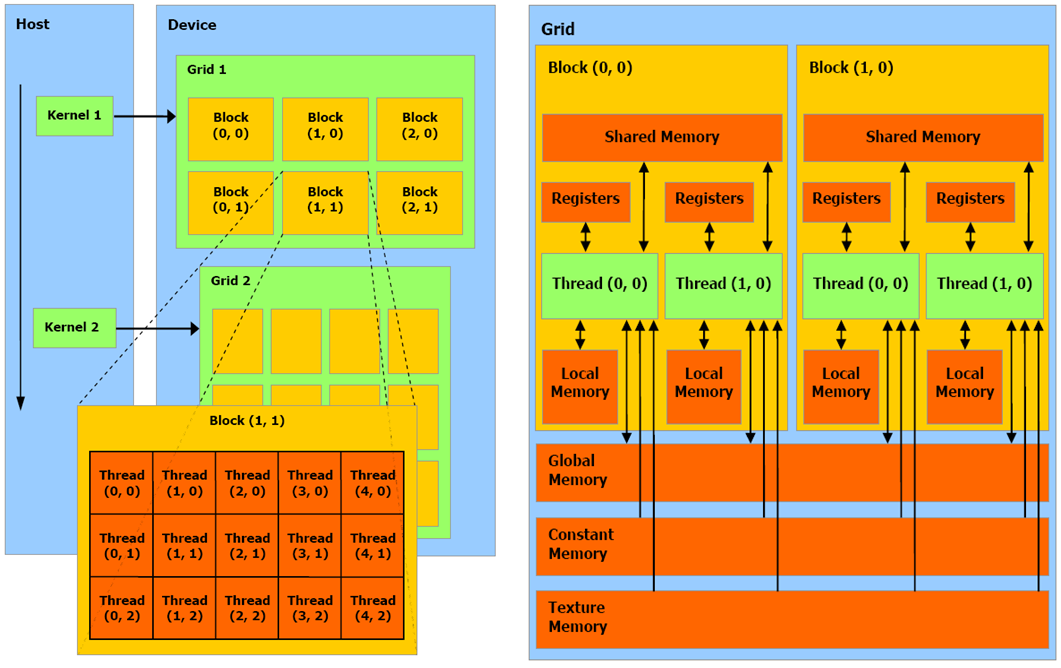
\includegraphics[width=\textwidth]{gpu2.png}
	\caption{CUDA layout and how the host CPU communicates information to the GPU when a kernel is invoked. (Adapted from http://geco.mines.edu/tesla/cuda\_tutorial\_mio/)}
	\label{fig:cuda}
\end{figure}

The CUDA kernel we created parallelize the calculation of forces onto the GPU.  As shown in Table~\ref{tab:profiling} later, this is the primary place where time is spent when performing these simulations.  In order to minimize the number of pairs that need to be evaluated when performing this calculation, we employ neighbor lists when performing GPU simulations.  The reason we use neighbor lists over cell lists is that each thread on the GPU is calculating the net force on a given particle.  This all the possible atoms that contribute must be locally available (local memory).  If we used cell lists, this number (per atom) could be far too large and we did not expect this to be efficient.  However, on the CPU cell lists are much easier to maintain and so are more efficient when such size concerns are irrelevant.  In both cases, a coherent memory pool makes maintenance of these lists easy. Therefore in both the GPU and CPU version of our code these lists are maintained on the CPU and hence the name of the class ``cellList\_cpu" (see cellList.h).  Although for the both the GPU and CPU versions of the code the name of the class does not change, in the former it is actually a neighbor list while in the latter it is a true cell list.  A preprocessor flag separates the two at compile time depending on whether the NVCC compiler flag is defined (see Makefiles for comparison).  This is one of many examples which illustrate the need for fundamentally different algorithms on GPUs than CPUs.

\subsection{Cell Lists}
On CPUs we maintain cell lists to minimize the number of pairwise comparisons each particle must check to compute the net force on each particle.  The easiest way to do this is by decomposing the simulation box domain into rectangular cells of size $r_s + r_{cut}$ where $r_{cut}$ is the cutoff in the pairwise potential and $r_s$ is the skin radius beyond this.  The use of a finite $r_s$ means that as the system evolve, the cell list does not need to be rebuilt (expensive) at every step.  Instead, one can simply check the net displacement since the last build of each particle.  If the sum of the two largest displacements exceeds $r_s$, then it is possible (if these displacements are antiparallel) that two particles which were not initially in each others' lists, now need to be (see cellList\_cpu::checkUpdate).  At this point the list must be rebuilt.  Full implementation details may be found in cellLists.cpp

A cell list is created the first time the force calculation is called.  This is comprised of two vectors in the cellList\_cpu class (which is a member of the virtual base class ``integrator") called ``head" and ``list" (private members of cellList\_cpu) which define a minimal linked list.
The head vector is a vector which contains the index of the ``first" atom in each cell.  This location is then iteratively looked up in ``list" which contains the index of the next atom in the cell.  The value located at that index in ``list"  provides the next, and so on until the value at a location in ``list" is 0 (in our C++ implementation we actually set this to be a negative number).  This is shown schematically in Fig.~\ref{fig:cell}.

\begin{figure}[H]
   	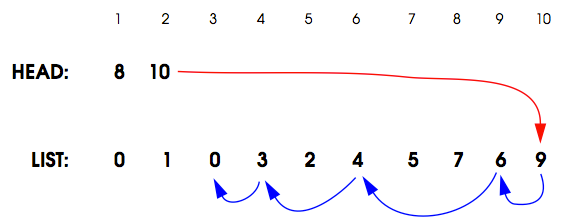
\includegraphics[width=\textwidth]{cell_list.png}
	\caption{Schematic of how our implemented cell lists work for the case of 9 atoms in 10 total cells, of which only cells 1 and 2 contain particles.}
	\label{fig:cell}
\end{figure}

The advantage of this technique is its simplicity; cell lists are easy to iterate through and only require $\mathcal{O}(N)$ space to store the information, where $N$ is the number of particles.  On a practical note, however, this iteration means that subsequent members of the list are not stored near each other in memory.  As a result, memory prefetching cannot be taken advantage of as cache misses become prevalent as N becomes large.  However, profiling has revealed that this is not too costly and we chose not to focus our efforts on changing this.
\subsection{Neighbor Lists}
On GPUs we maintain a neighbor list for each atom.  This neighbor list again keeps a record of all other atoms that are within $r_s + r_{cut}$ of each atom.  The addition of a finite skin radius again means the neighbor lists do not need to be rebuilt at every time step. If this radius is too large, each atom checks an excessive number of neighbors at each integration step, however, if it is too small the lists must be rebuilt more often.  We investigated the effects of changing this radius systematically as discussed in detail in following sections.

These lists are stored as two linear arrays called ``nlist" and ``nlist\_index" (see cellList.cpp).  Element $j$ of the latter contains the index of the former where the information pertaining to the neighbors of $j$ is located.  At nlist[j] is an integer which is the number of neighbors, $n$, atom $j$ has, whose indices are recorded in the following $n$ elements of nlist (see Fig.~\ref{fig:nlist}).  This linear storage is optimal for passing it to the GPU.  These lists are built and maintained on the CPU since, when being built, every atom must be compared to every other one ($\mathcal{O}(N^2)$ process) which we deemed to be far too much communication for the GPU to handle locally on the device.

\begin{figure}[H]
   	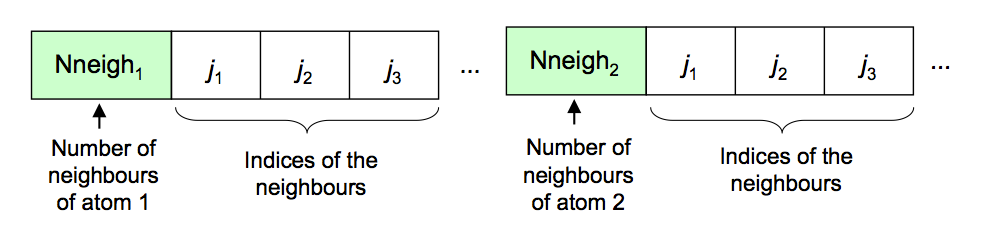
\includegraphics[width=\textwidth]{nlist.png}
	\caption{Schematic of how our implemented neighbor lists work.  Above is a depiction of nlist, while nlist\_index contains the indices of the green cells.}
	\label{fig:nlist}
\end{figure}

In fact, in very advanced codes such as HOOMD (http://codeblue.umich.edu/hoomd-blue/)~\cite{Anderson2008}, the neighbor lists themselves may be maintained on the GPUs.  This \emph{significantly} improves the speed of the code because it reduces the number of times data (memory) has to be sent back to the CPU. However, this requires communication between threads outside different blocks, various clever reductions, and a very careful consideration of the cache coherency on the GPU.  As a result, it is (unfortunately) well beyond what we found feasible in the time-frame allotted for this project, though we did investigate this in the literature~\cite{Lipscomb2012}. As will be shown in the following sections, this communication loss actually makes the GPU code slower than it can be, even though we will show that it overall is faster than our CPU code and significantly improves the speed of the force calculation, which were major deliverables of this project.

\subsection{Testing}

We implemented Google Tests within our software (see Makefile TESTS, and unit tests.cpp) to ensure our code was functioning properly.

We implemented the following tests:
	\begin{itemize}
	\item[\texttt{NumAtoms}] verifies that the system class stores the correct number of atoms
	\item[\texttt{KineticEnergy}] calculates the kinetic energy for a two-atom system, and verifies that it is correctly returned by the KinE() function
	\item[\texttt{PotentialEnergy}] calculates the potential energy for a two-atom system, and verifies that it is correctly returned by the PotE() function
	\item[\texttt{ChangeBox}] changes the length of the simulation box and verifies that the box is correctly changed in the system definition
	\item[\texttt{PBC}] computes the distance between two particles using the minimum image convention and verifies that it is correctly computed for different scenarios (out of box, inside box, etc.)
	\end{itemize}

Additionally, we benchmarked/validated our code's results against LAMMPS \cite{Plimpton1995}, described later in this report.

\section{Code Structure and Implementation Notes}

The software is implemented in object-oriented C++ and version-controlled through an actively updated github repository \url{https://github.com/PrincetonUniversity/CBEMDGPU}. The code is completely documented using \textbf{Doxygen} in the /doc directory, which contains both an html and a pdf document (doc/output/latex/\textbf{refman.pdf}) outlining the code structure and commenting all of the functions in the software.
%
The code structure is briefly summarized as follows:
\begin{description}

\item[\texttt{common.h}] This file contains classes that implement the error catching functions.

\item[\texttt{cudaHelper.cu/.h}] This file contains classes that assist in communicating with, and tuning, the GPUs.

\item[\texttt{cellList.cpp/.h}] This file contains the class which controls the cell lists (for parallelization on CPU) or neighbor lists (for parallelization on GPUs).

\item[\texttt{dataTypes.h}] This file contains custom data structures, such as the ``atom" structure, which stores the position, velocity, and acceleration of an atom, and identical structures like int3 and float3 which are implemented by default on the GPU.  For consistency, we use identical structures in our CPU version as well, however they require an explicit definition which is provided herein.
	
\item[\texttt{integrator.cpp/.h}] This file contains the ``virtual'' base class which is the parent of all integrators we implemented (NVE and NVT with Nos\'{e}-Hoover)

\item[\texttt{integrator.cu}] This file contains all potential functions, kernels, etc. required for the GPU implementation of our code.

\item[\texttt{nve.cpp/.h}] This file contains the integrator class which implements the velocity-Verlet integration scheme for an NVE simulation.

\item[\texttt{nvt.cpp/.h}] This file contains the integrator class which implements the velocity-Verlet integration scheme with a time-reversible Nos\'{e}-Hoover thermostat for an NVT simulation.

\item[\texttt{potential.cpp/.h}] The file contains the potential class which implements the force and potential energy calculations for the standard Lennard-Jones potential.

%
This class can be expanded to include other potential energy functions.

\item[\texttt{system.cpp}] This file contains the class which stores all of the parameters relevant to the simulation system, such as the box size, potential energy function, and the number of atoms.

\item[\texttt{utils.cpp}] This file contains the necessary ``helper'' functions for the simulation, such as the distance calculation with periodic boundary conditions using the minimum image convention.

\item[\texttt{main.cpp}] This is the main driver program to run the software.

\item[\texttt{unittests.cpp}] This file implements Google Tests for our software.
%
We used a test fixture to initialize the same system construct for multiple tests.

\end{description}

\subsection{Optimizations}
This section provides an overview of the optimizations performed in our software to lead to the final submitted version.  Iterative profiling was performed during development to prove these led to speed improvements, generally on the order of 5-20\% each between successive iterations.  The principle optimization tool was the use of OMP wherever possible, though intelligent C/C++ programming techniques also led to expected improvements. We outline the major optimizations employed in each file here.

\begin{description}

\item[\texttt{cellLists.cpp}] In order to maintain the cell and neighbor lists on the CPU efficiently we implemented a number of optimizations in the cellList\_cpu class, mostly in the cellList\_cpu::checkUpdate method which is responsible for checking whether the lists need to be updated.  Most algorithms we found in textbooks and in the literature simply state that if any pair of particles move toward each other more than the skin radius added to the cutoff radius of the potential used to build these lists, then the lists must be rebuilt.  This implies checking all pairs of particles which is an $\mathcal{O}(N^2)$ expense.  In fact, it is clear that this can be made truly $\mathcal{O}(N)$ by simply storing the positions of each atom at the time the lists are constructed, then calculating the displacement from those positions at each step. The largest two displacement magnitudes are then recorded (which does not require a full sorting of all the displacements, which is, in itself, an improvement). If one always assumes the worst possible scenario, that is, these two displacements are antiparallel, then if the sum of the displacements exceeds the skin radius, the lists should be reconstructed.  We employ this for both the CPU (cell lists) and GPU (neighbor lists) implementations.  This assumption is more restrictive than if each pair were truly calculated, especially since no assumption about the direction of each displacement is necessary, however this requires $N^2$ calculations each of which involve taking a square root which is very costly.  By making this blind, worst case scenario assumption, in fact we find that the code speeds up between 5 and 20\% depending on the system depending on the density, cutoff and skin radius, etc.

On the GPU, where we implement neighbor lists, we also use some basic tricks of memory allocation to speed up the creation of the list.  As previously discussed, this must be a linear array in memory so they cane sent efficiently to the GPU.  However, since the number of neighbors changes, so does the size of each region between the green colored indices in Fig.~\ref{fig:nlist}. In fact, we preallocate a 2D array with space for each particles neighbors, into which each the list is built initially.  However, instead of simply appending each dimension every time an additional neighbor is found (beyond what was initially allocated in the 2D array), that list is doubled in size each time a new neighbor would otherwise overflow the current list.  Afterward the list is trimmed and linearized.  This dramatically reduces the number of memory operations and led to an estimated speed up of 10\%.

Such considerations were not necessary on the CPU since the ``head" and ``list" arrays (linked lists) are constant in size.  However, because of the memory operations for neighbor lists and the iterative nature of linked lists, neither list construction could be parallelized with OMP.  For true cell lists on the CPU, each cell must be linked to each of its neighbors so their constituent atoms could be compared.  Precomputing this, rather than on the fly led to another increase in speed of about 15\%.

\item[\texttt{integrator.cpp}]
The integrator::calcForce member of the virtual base class ``integrator" calculates the pairwise forces for all atoms in the simulation.  It first calls the checkUpdate member of its private cell list to see if the list needs to be updated, then proceeds to calculate the forces by comparing all the particles in a cell with those in the neighboring cells.  The cell width (skin radius plus the potential cutoff) is such that all particles within these neighbors are the only particles that need to be compared with those in the central cell.  Thus the loop executes by going cell by cell through the list.  OMP can be exploited to parallelize this and to compute the total potential energy simultaneously by using an ``omp parallel reduction" clause.  Dynamic scheduling was found to be the fastest (marginally since the system's density was generally homogeneous) with a chunk size of 1.  Because each thread is comparing all particles in a cell to all of those in the neighboring cells, a chunk size of 1 was actually found to be optimal.

In addition, since the instantaneous accelerations of each atom is the result of a sum over all pairwise interactions, we stored the accelerations in a separate vector rather than storing them locally in each atom structure.  This is because the instantaneous accelerations would otherwise have to be set to zero initially before each integration step which becomes a significant cost once the simulation incorporates many thousand of atoms.  OMP can then be used to assign these after the loop has finished, which gave us optimal performance.  Such considerations were irrelevant in the GPU implementation.

\item[\texttt{integrator.cu}]
The GPU functions necessary for our simulation must be compiled with NVIDIA's nvcc compiler which only recognizes .cu extensions.  As a result, we placed all the necessary functions to parallelize the force calculation in this file.  ``Device" analogs of functions that otherwise would execute on the host in the CPU version are indicated with ``dev\_" prefixes.  This includes dev\_pbcDist2, dev\_pairUF, and dev\_slj.  These include similar optimizations as applied to their CPU counterparts which are discussed in the following sections, so we will not repeat them here.  The GPU kernel ``loopOverNeighbors" is discussed in Section~\ref{sec:gpukernel} which we also neglect for the moment.

The primary ``optimizations" which we implemented in the GPU version of integrator::calcForce come simply from the use of the thrust library.  As previously discuss, thrust is a library which extend STL-like functionality from the CPU to the GPU (vectors, iterators, etc.) and most importantly, introduces the concept of scoping.  Traditionally, when before a GPU kernel is called, memory must be allocated, data sent to that location, then the kernel is executed, and memory must be deallocated afterwards.  However, with scoping, the deallocation is handled automatically preventing memory leaks.  Furthermore, the use of ``device\_vectors" automatically allocates memory on the GPU device which can be directly filled with (relatively) fast memcpy (memory copy) commands behind the scenes.

Technically, the kernel cannot be invoked with a direct pointer to the host side device\_vectors so a pointer to the GPU device memory location must be used instead.  Fortunately, thrust provides a built-in function called ``thrust::raw\_pointer\_cast" which produces this automatically.  Refer to the code for examples of how this is implemented.  Following the kernel call, which computes all the forces
on each atom, the data can be collected back on the host CPU with a simple copy command and the total potential energy can be found by using a ``thrust::reduce" call which is similar to its OMP counterpart (which also helps speed up the calculation).  We found that a block size of roughly 512 threads per block was optimal, and this is automatically set in main.cpp, though for smaller GPUs the block size is detected and checked with the help of the class (and subsequent members of) systemProps in cudaHelper.cu

As will be pointed out later, our GPU code was faster overall than our CPU code, but had reductions in total possible speedup since this memory allocation and deallocation had to occur at every time step in the simulation.  We did not believe this would turn out to be such as issue so we initially designed the CPU code to be commensurate with this sort of parallelization of the force calculation by separating the force calculation and integration steps into different classes.  Given more time, we suspect that one improvement would come from actually performing the integration step directly on the GPU.  However, even then the system would have to be returned to the CPU host to maintain the neighbor lists.

Highly optimized codes are actually capable of maintaining these lists directly on the GPU and so do not suffer from these problems.  However, after investigation into the literature and source code of available examples~\cite{Anderson2008, Lipscomb2012} we soon realized this is a non-straightforward task; one which has been the subject of a number of recent research articles and is still an active area of research in computer science.  Unfortunately, this was well beyond what we could implement in a semester project, but the reasons for our code's slow overall performance are well understood.  Nevertheless, the force calculation itself was accelerated thanks to the GPUs as discussed later (see Section~\ref{sec:scalingstudies}).

%add bit about slj singularity protection

\item[\texttt{nve.cpp and nvt.cpp}]
Both of these integrators make straightforward, extensive use of OMP parallelization to perform the necessary calculations.  Both reductions and ``parallel for" clauses were very useful.  Dynamic scheduling with a chunk size of 100 was found to be roughly optimal in most cases, hence we defined the OMP\_CHUNK macro in common.h to reflect this, which is used by default for these loops whenever possible.

\item[\texttt{potential.cpp}]
Two pair potentials are actually provided in this file; one is called ``pairUF" which is the potential from the last homework assignment (which was used as another test to verify our code worked properly) and the shifted Lennard-Jones (``slj").  The implementation of the latter was the primary goal of this project, however, we tested and implemented both.  Basic optimization generally apply to both cases and were a fruitful endeavor since the potential calculation constitutes a significant fraction of the overall simulation time.  After the following optimizations the total time spent in these routines dropped by about 10\% overall (see Table~\ref{tab:profiling}).

To begin, the pair potential is zero if two atoms are beyond a certain cutoff distance and require no computational effort; using the square of this to compare before any calculation is performed is actually faster since when the distances are computed (see utils.cpp) the distance function can avoid taking an expensive square root.  Furthermore, precomputing factors which are constantly reused led to increased performance.  This was particularly noticeable for cases where we replaced quotients with products, that is, replacing a division by $x$ with a multiplication by $1/x$, at least when compiling the g++ compiler.  The intel compiler (icpc) actually seemed intelligent enough to replace this automatically when optimization flags were specified at compile time and we saw no significant change, though we left the code with the hard-coded improvements anyway.  In addition, the slj function must take certain quotients to the powers of 12 and 6; replacing this with products (say x2 = x*x; x6 = x2*x2*x2; x12 = x6*x6) also led to noticeable improvements in some cases.

\item[\texttt{system.cpp}]
This file contains the methods for the systemDefinition class.  These routines are involved in start-up and tear-down of the simulation and are not called on a regular basis except systemDefinition::writeSnapshot (which prints instantaneous snapshots of the system to a file).  As a result optimizations were not typically employed here, though we did use an OMP statement in systemDefinition::initRandom (creates a random initial condition) just to illustrate the point.  We did, however, make use of the boost library's ``normal\_distribution" to generate initial velocities according to a Maxwell-Boltzmann distribution which helps the system reach equilibrium faster during simulation.

\item[\texttt{utils.cpp}]
The functions in this file pertain to handling the so-called ``minimum image" convention used in simulations with periodic boundaries.  The ``minimum image distance" is the distance between the two nearest periodic images of a pair of atoms.  Often the ``real distance" is initially computed by simply subtracting the two coordinates to obtain a vector, then each dimension is reduced by L*floor($dx$/L), where $dx$ is the component of the vector in a given principle cartesian direction and L is the box length in that direction.  While general, the floor function is costly and can be replicated with while loops as illustrated in the functions ``pbc" and ``pbcDist2."  In the latter function, for reasons previously discussed, we also choose to return the square (magnitude) of the minimum image distance to avoid taking a square root uneccessarily.

\end{description}

\subsection{The GPU Kernel}
\label{sec:gpukernel}
The CUDA kernel we invoke is called ``loopOverNeighbors" in integrator.cu; this function takes a linear array of atoms, a neighbor list, and
a few other parameter inputs and returns the force experienced by each atom in the simulation.  A thread for every atom is executed, organized into chunks called ``blocks" on the GPU.   This kernel is what each thread in each block  on the GPU is performing.   Since the total number of atoms is, in general, not evenly divisible by the blocks size (512 as previously discussed), a check is first performed to ensure that the thread executing these instructions corresponds to an atom in the system.  For example, a system of 1200 atoms will have to employ 3 blocks of 512 threads each, though the last one will be largely empty.  The thread identification index (called ``tid" in the code) is first calculated based on the size of each grid (blockDim.x), the current grid the thread is residing in (blockIdx.x) and the local thread index within that block (threadIdx.x), such that

\begin{equation}
	tid = threadIdx.x + blockIdx.x*blockDim.x
\end{equation}

Once this identification is made, one simply iterates through the neighbor list, calling the pair potential function on each atom in the list relative to this atom (index tid).  Refer to the loop in integrator.cu for more implementation details.  In order to identify which potential function to use, in the anticipation of future extensibility, we explicitly send a flag to the kernel (pFlag) which indicates which one to select.  The alternative we investigated was to formally bind the memory location of the device function equivalent to the host CPU's potential function (as a pointer to device memory) to a variable which can be passed as the kernel is called; however, we were unable to obtain consistent results, likely due to some memory management issues behind the scenes so we opted to use a simpler route.

We point out that the way the neighbor list is organized is not very cache-coherent, that is, each time new atoms must be found in the list (global memory) and thus loaded into the local registers, they are not guaranteed to be ``close" to other atoms in the same list.  So hierarchical memory management does not usually assist this process.  In highly optimized simulations, very advanced cache-sorting routines are employed to sort the list based on atom positions which helps the GPU take advantage of keeping the same data in the local registers for longer, thus improving their performance.  However, such routines do not always produce a speed up, since the cache-coherency is still only approximate when such sorting is applied and the overhead for doing so is not trivial.  Due to its level of sophistication, our limited time,  and minimal promised gains we did not pursue this for our own code, though in the future this could be added.

\section{Results}

\subsection{Profiling}

Profiling was performed on the TIGER computer cluster using gprof with a number of different processor, skin radius, and particle combinations. We found that using 4 processors, 400 particles, a skin radius of 0.5 for 100 steps produced the most representative results. The software was compiled using the \textit{-pg} compiler option. The top 7 most expensive components of the software are presented in Table~\ref{tab:profiling}.

% Table generated by Excel2LaTeX from sheet 'Sheet1'
\begin{table}[htbp]
  \centering
  \tiny
  \caption{Profiling results of our code in terms of most expensive functions, in order.}
    \begin{tabular}{ccccccc}
    \toprule
    \% time & Cum Seconds & Self Seconds & \# of Calls & Self (s/call) & Total (s/call) & Name \\
    \midrule
    26.86 & 1.3   & 1.3   & 101   & 0.01  & 0.05  & integrator::calcForce(systemDefinition\&) \\
    17.05 & 2.13  & 0.83  & 6125941 & 0     & 0     & pbcDist2(float3 const\&, float3 const\&, float3\&, float3 const\&) \\
    15.5  & 2.88  & 0.75  & 34484119 & 0     & 0     & std::vector<float3, std::allocator<float3> >::operator[](unsigned long) \\
    10.74 & 3.4   & 0.52  & 5702835 & 0     & 0     & slj(float3 const*, float3 const*, float3*, float3 const*, float const*, float const*) \\
    8.27  & 3.8   & 0.4   & 10997635 & 0     & 0     & cellList\_cpu::list(int) const \\
    7.23  & 4.15  & 0.35  & 11617957 & 0     & 0     & std::vector<int, std::allocator<int> >::operator[](unsigned long) const \\
    4.75  & 4.38  & 0.23  & 12810108 & 0     & 0     & std::vector<atom, std::allocator<atom> >::operator[](unsigned long) \\
    \bottomrule
    \end{tabular}%
  \label{tab:profiling}%
\end{table}%

The \textbf{calcForce} function consisted of the most expensive function in the program, followed by \textbf{pbcDist2}. The function calls to the shifted lennard-jones \textbf{slj} potential and cellLists that are maintained on the CPU \textbf{cellList\_cpu}. It would be expected that the \textbf{calcForce} function utilizes the majority of the computing time and this has been observed elsewhere in MD codes. Due to the expense of this function, this function was parallelized on the GPUs.

\subsection{Scaling Studies}
\label{sec:scalingstudies}

We performed several scaling studies on the TIGER cluster for CPUs and ANDROS/TIGER for GPUs. Runs were performed on 1,2,4,8, and 16 processors on tiger, for $r_{s}$ (skin) cutoffs of 0.00, 0.50, and 1.00 and for 1000, 2000, 4000, 8000 particles for 10,000 steps. We used the shifted Lennard-Jones potential with parameters $\sigma = 1.0$, $\delta = 0$, $U_{shift} = 0.0$, and $\epsilon = 1.0$ where the cutoff radius ($r_c$) was set to 2.5$\sigma$.  The system box size was set to the cube root of the number of particles to maintain a fluid-like density.  The scaling results are shown in Figure~\ref{fig:scaling_compare}.  

\begin{figure}[H]
	\begin{subfigure}{0.5\textwidth}
    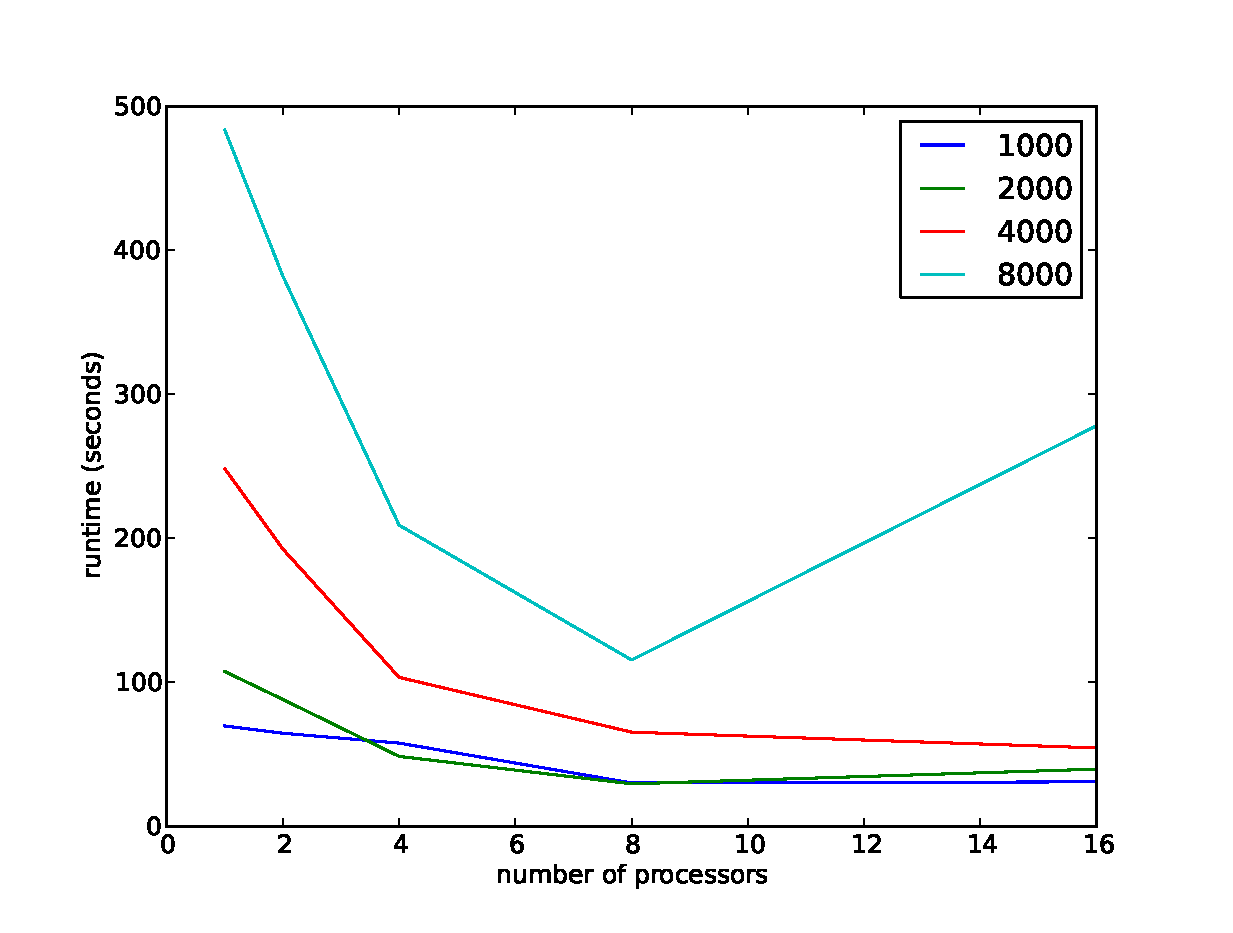
\includegraphics[width=\textwidth]{scalingtiger_rs_000}
	\caption{}
	\end{subfigure}
	\begin{subfigure}{0.5\textwidth}
	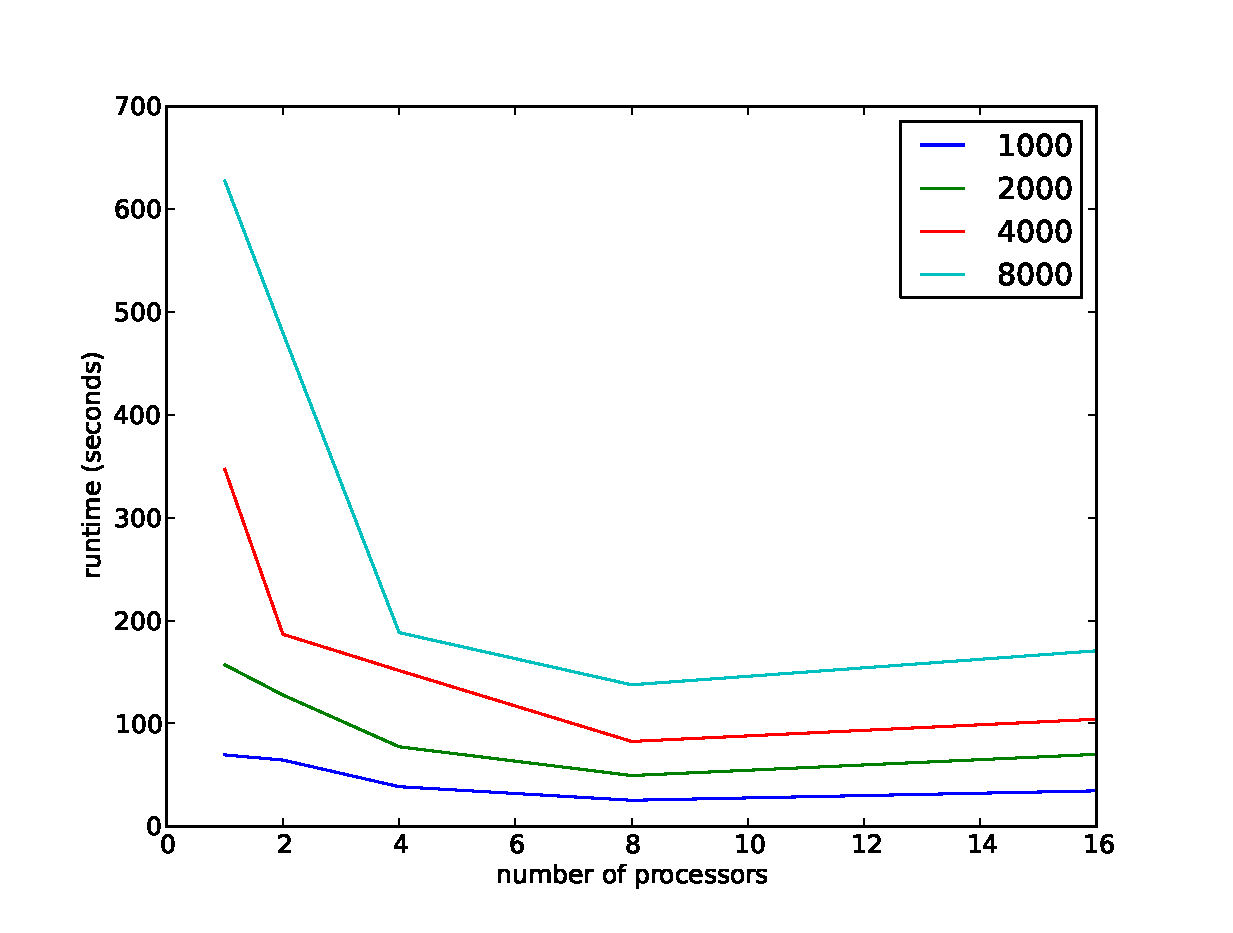
\includegraphics[width=\textwidth]{scalingtiger_rs_050}
	\caption{}
	\end{subfigure}
	\begin{subfigure}{0.5\textwidth}
	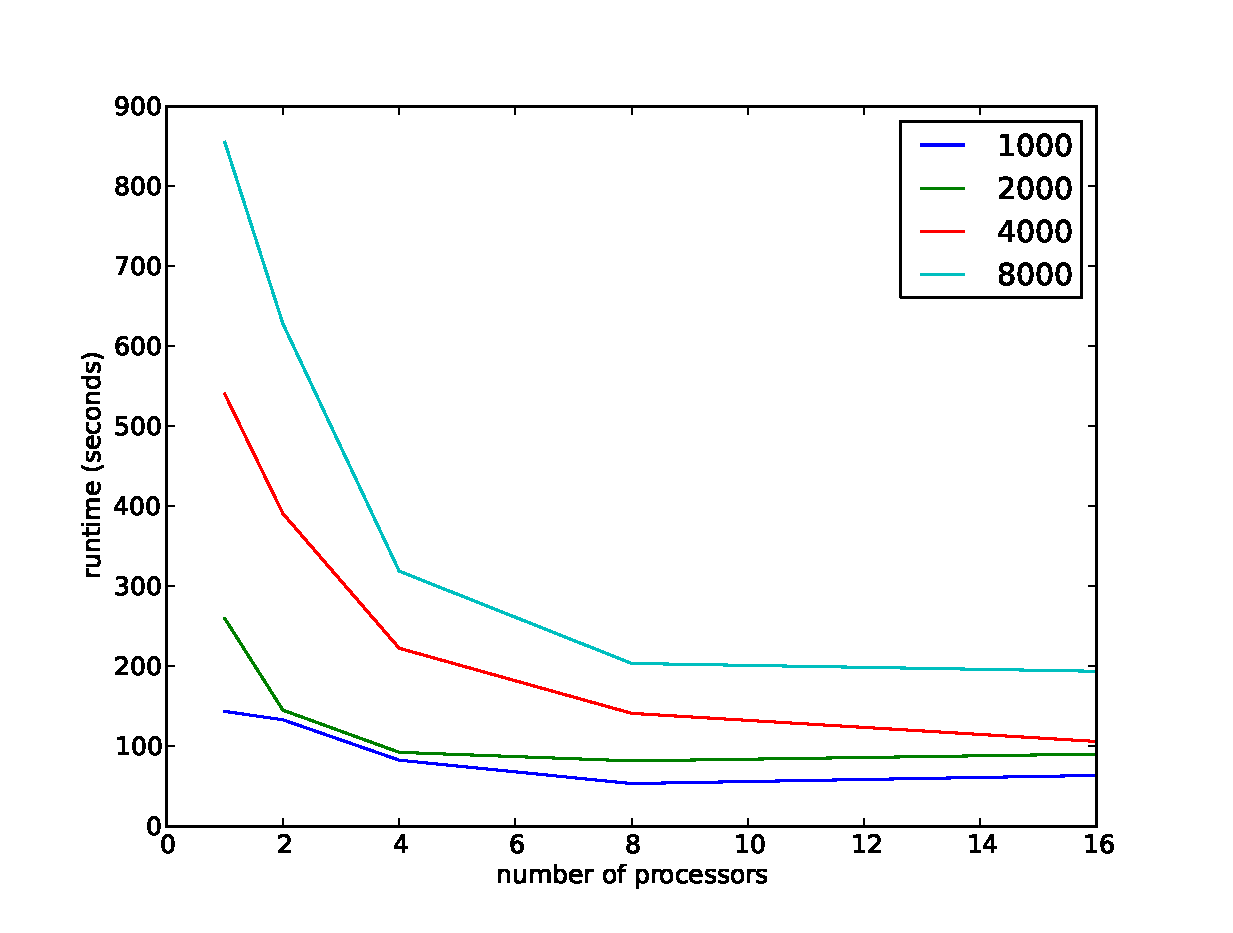
\includegraphics[width=\textwidth]{scalingtiger_rs_100}
	\caption{}
	\end{subfigure}
	\begin{subfigure}{0.5\textwidth}
	\includegraphics[width=0.7\textwidth, angle=-90]{gpu_time.eps}
	\caption{}
	\end{subfigure}
	\caption{Scaling results from testing our molecular dynamics simulations on CPUs and GPUs for different combinations of particle numbers, $r_{s}$ values, and number of processors. (a) $r_{s}$ = 0.00 (b) $r_{s}$ = 0.50 (c) $r_{s}$ = 1.00 (d) Scaling on the GPU when the CPU fraction of the code used 1 and 4 processors compared to the CPU results on a single core at various skin radii.}
	\label{fig:scaling_compare}
\end{figure}

We observed that for all particle numbers introducing more processors scaled the requisite simulation time down relatively well, except for the case of $r_{s} = 0.00$. Note that in this case, the simulations nearly always finished sooner than their corresponding simulations when $r_s > 0$.  When the skin radius is zero, the cell lists are rebuilt every time and no maintenance (checkUpdate routine) needs to be done.  In fact, this reveals that the maintenance cost for cell lists on these systems outweighs their advantages for (relatively) small numbers of particles.  Adjusting the chunk size for OMP did not lead to qualitative changes in these trends.  However, we expect that for extremely large systems, this would no longer hold.  In the case of $r_s = 0$ for 16 processors with 8,000 atoms some communication issues arose on TIGER's hardware and led to poor scaling.  

On the GPU we found that our simulations were sped up by about 30-50\% over their CPU counterparts on a single processor for smaller system sizes.  This is an impressive step forward given that the only thing we parallelized was the force calculation which comprises only about 27\% of the cost in the CPU implementation (see Table~\ref{tab:profiling}).  However, given that we additionally deployed device functions for the ``slj" and ``pbcDist2" on the GPU we were also able to cut into how much time each of these functions contributed to the overall speed of the program.  Thus we found that our GPU code performed quite admirably in this regime.  The size of the skin radius had negligible effect on the GPU code's speed so the results in Fig.~\ref{fig:scaling_compare} are representative for $r_s = 0,0.5$, and 1.  This is not uncommon for neighbor list implementations.  We also tested the case of having a different number of processors available for the (albeit small) fraction of the GPU code's use of the CPU to perform additional tasks.  As evidenced, this is negligible so it made almost no difference going from 1 to 4 processors.  Compared to the purely CPU code on a single core, the GPU code was up to twice as fast for a small number of particles when using large skin radii.  However, as shown by the fitted curve, the GPU time scales as $N^2$.  This is because of its reliance on neighbor lists (which is $\mathcal{O}(N^2)$) rather than cell lists ($\mathcal{O}(N)$ expense).  For the system sizes we investigated this did not present an advantage because our systems were small enough that, it is likely cell lists could be feasibly implemented on the GPU.   However, it is known that for large systems this becomes untenable due to bandwidth limitations~\cite{Anderson2008, Lipscomb2012} which is why we chose not pursue this.  This simply emphasizes the importance of maintaining these lists directly on the GPU, though for reasons already discussed, we were not able to implement such a routine.

\subsection{Benchmarking and Validation against Literature Values}

\begin{table}[H]
\begin{centering}
	\begin{tabular}{| r | c | c |}
		\hline
		 & CBEMDGPU & LAMMPS \\
		 \hline
		 T & 0.7104 & 0.7112 \\
		 \hline
		 Potential energy / atom & -5.6532 & -5.6594 \\
		 \hline
		 Total energy / atom & -4.5879 & -4.5929 \\
		 \hline
	\end{tabular}
	\caption{Comparison of average thermodynamic quantities for CBEMDGPU and LAMMPS simulations.}
	\label{table:lmp_compare}
\end{centering}
\end{table}

We validated our code against LAMMPS \cite{Plimpton1995} (http://lammps.sandia.gov), an existing and widely-used and tested commercial molecular dynamics software package.
%
We simulated a system of 4000 Lennard-Jones particles at a reduced temperature $T=0.71$.
%
We used a cubic box with edge length $L=16.796$, so that the reduced density of the system $\rho = 0.8442$.
%
We used a timestep $\Delta t=0.005$, and simulated for $10,000$ timesteps.


We compared the temperature, potential energy, total energy, radial distribution function, and mean squared displacement for the simulations calculated in our package against LAMMPS.
%
The results are shown in Figure~\ref{fig:lmp_compare} and Table~\ref{table:lmp_compare}.
%

\begin{figure}[H]
	\begin{subfigure}{0.5\textwidth}
    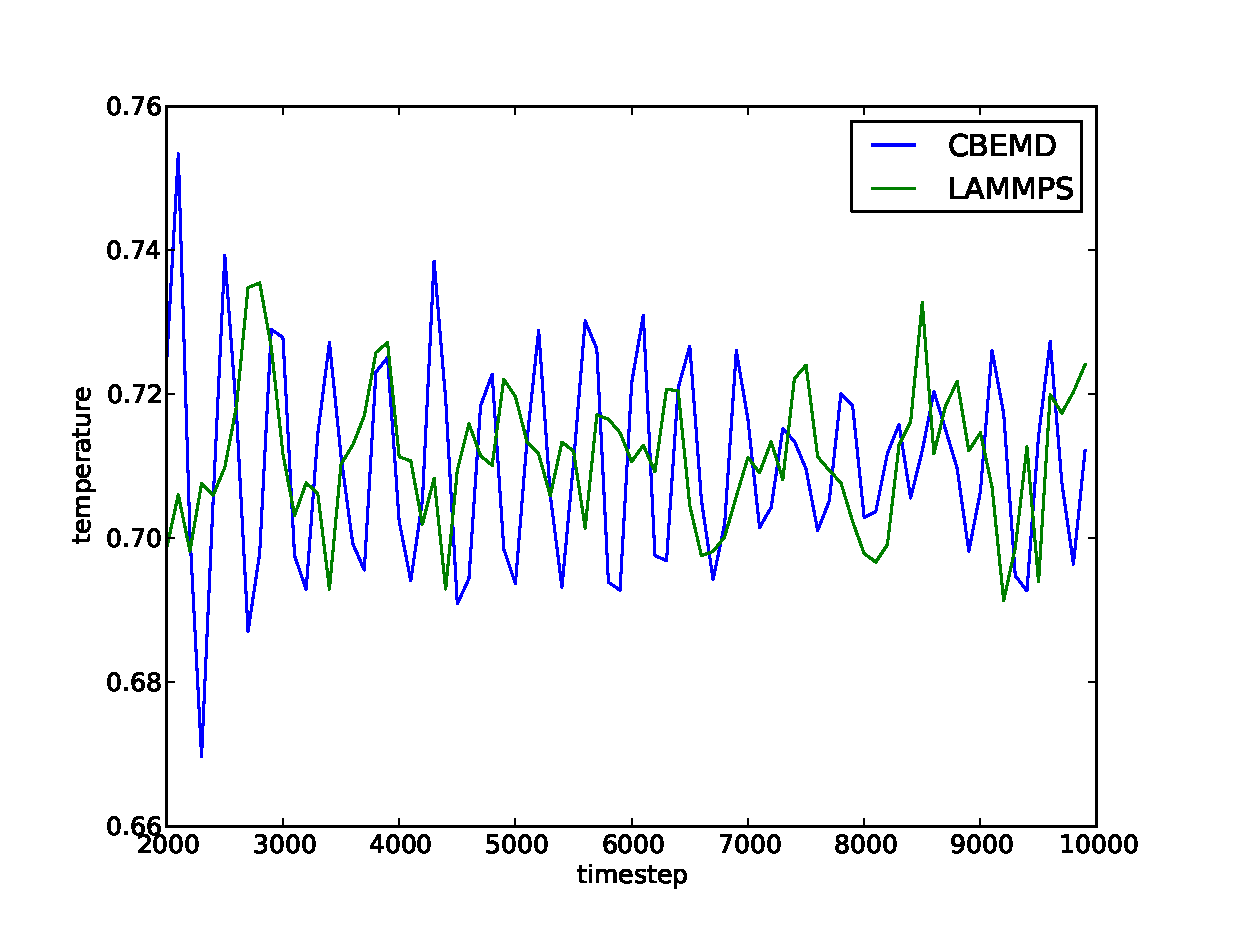
\includegraphics[width=\textwidth]{T_compare}
	\caption{}
	\end{subfigure}
	\begin{subfigure}{0.5\textwidth}
	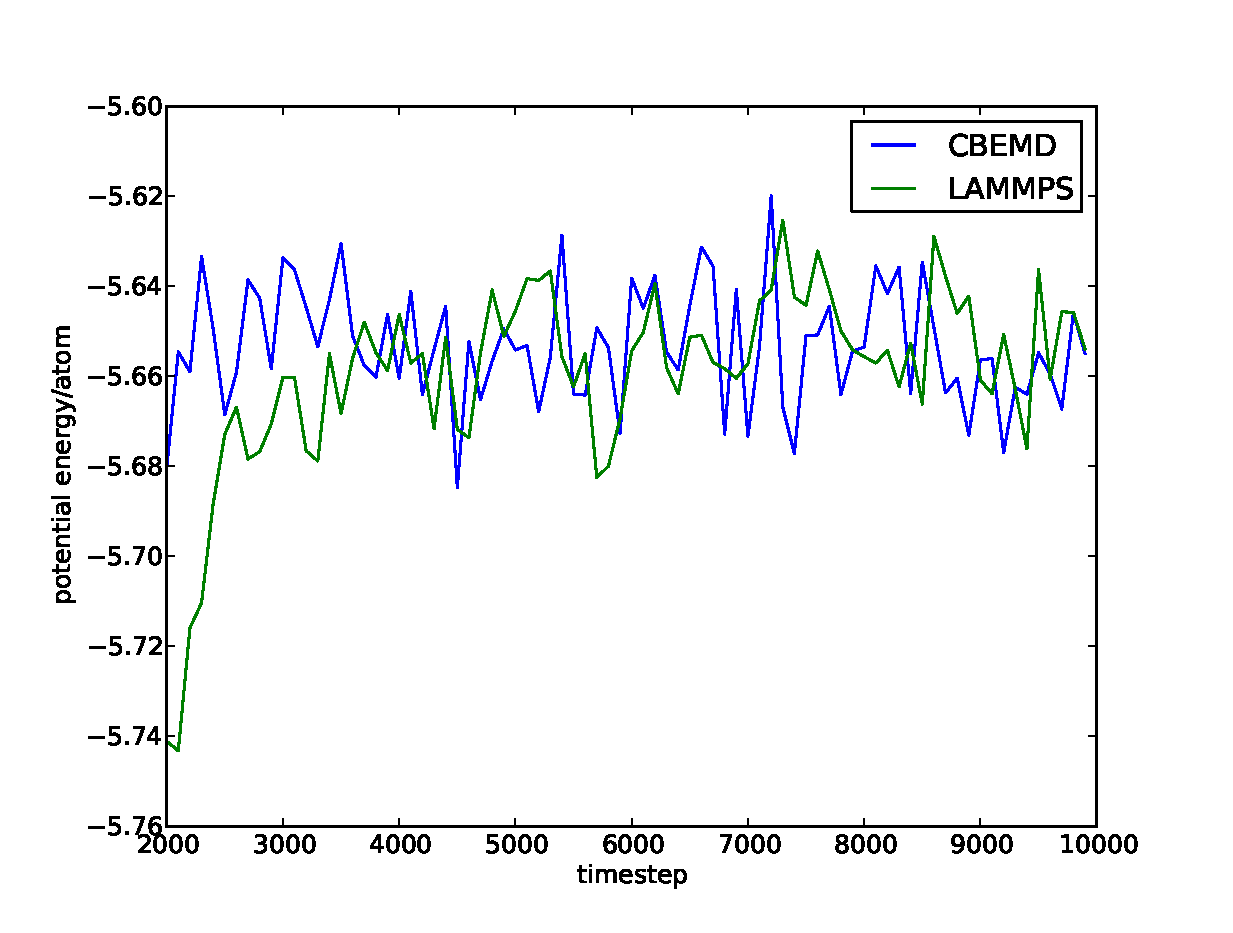
\includegraphics[width=\textwidth]{PE_compare}
	\caption{}
	\end{subfigure}
	\begin{subfigure}{0.5\textwidth}
	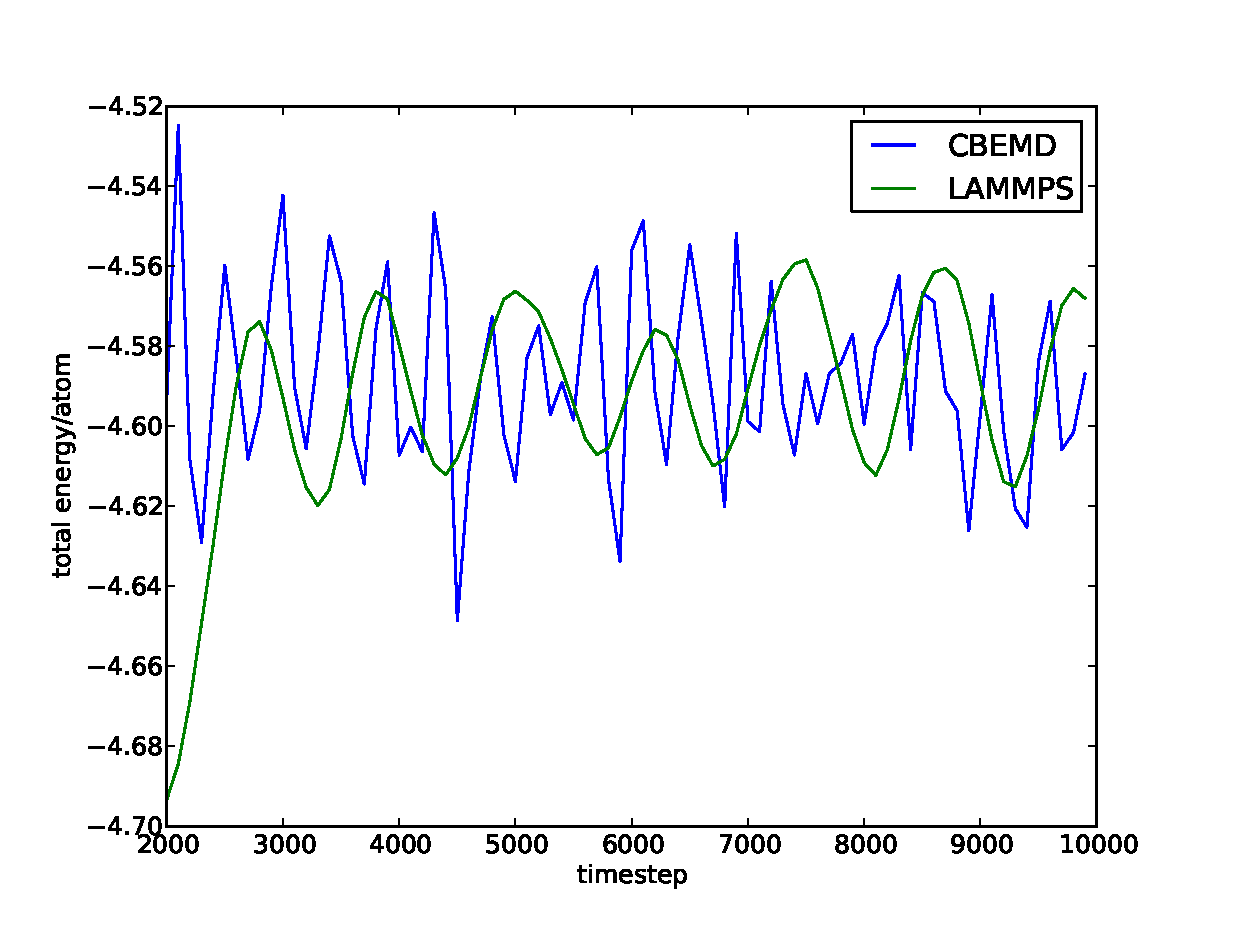
\includegraphics[width=\textwidth]{E_compare}
	\caption{}
	\end{subfigure}
	\begin{subfigure}{0.5\textwidth}
	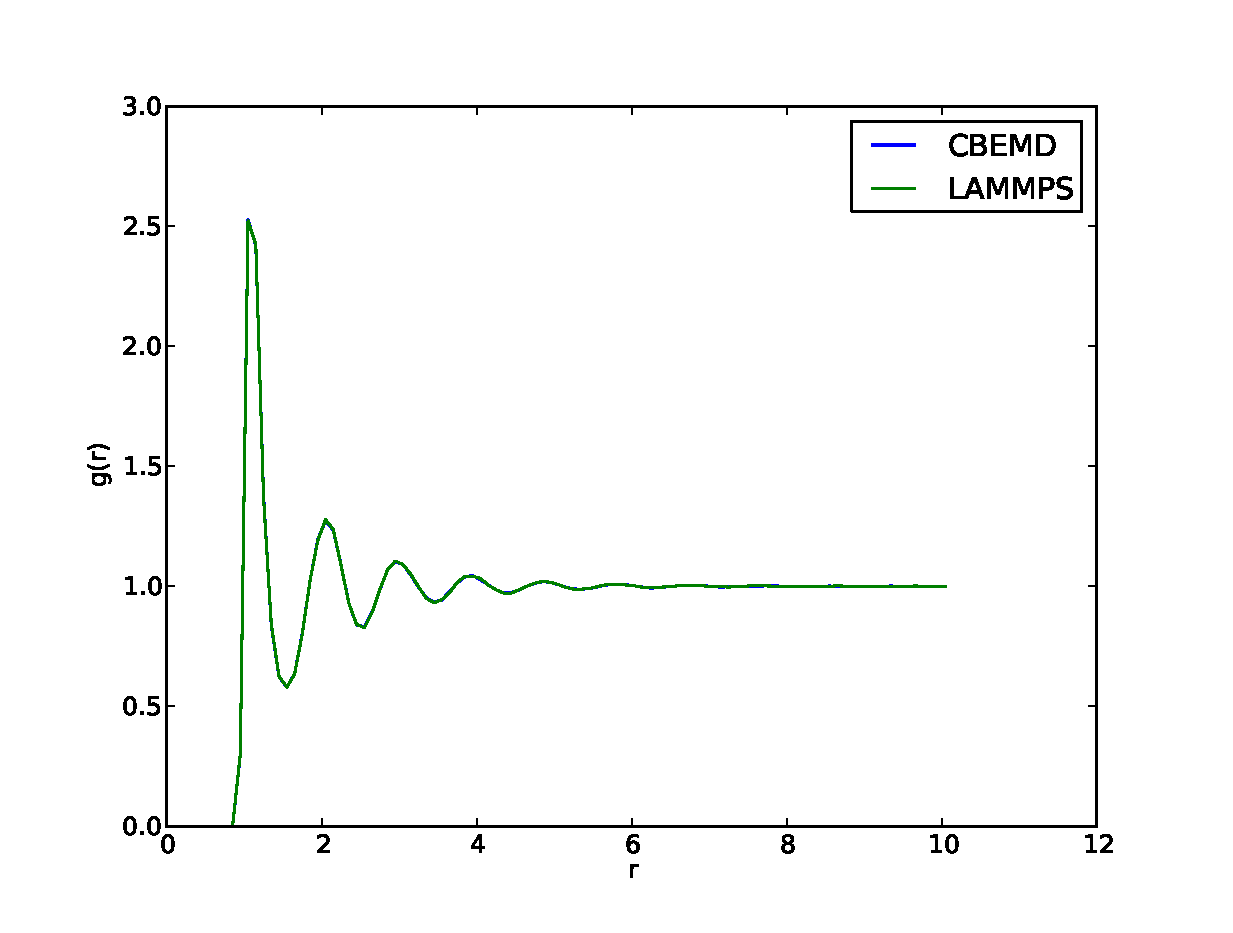
\includegraphics[width=\textwidth]{gr_compare}
	\caption{}
	\end{subfigure}
	\begin{subfigure}{0.5\textwidth}
	\includegraphics[width=0.65\textwidth, angle=-90]{msd.eps}
	\caption{}
	\end{subfigure}
	\caption{Comparison between CBEMDGPU simulation and LAMMPS simulation for 4000 Lennard Jones particles at $T=0.71$ and $\rho=0.8442$. (a) Comparison of temperature over time. (b) Comparison of potential energy/atom over time. (c) Comparison of total energy/atom over time. (d) Comparison of radial distribution functions. (e) Mean squared displacement of atoms over normalized time; we report results well into the diffusive regime, as evidenced by the slope of unity in log-log scale.  Anticorrelation (from collisions) following the ballistic regime are responsible for the poor fit at short times as well as the local reduced slope.}
	\label{fig:lmp_compare}
\end{figure}

There is excellent agreement between our software (CBEMDGPU) and the LAMMPS results. The average temperature and the behavior of the temperature fluctuations were qualitatively and quantitatively in agreement. Our temperature fluctuations are more smooth since we don't have as much damping and since LAMMPS uses Nos\'{e}-Hoover \emph{chains} whereas we use a single ``spring" to dampen the fluctuations. The potential and total energies' behaviors are the same, and the radial distribution functions calculated in both programs are within numerical error. These results illustrate that the software we have developed can reproduce the thermodynamic and dynamic behavior of the LAMMPS software, and is a strong validation of our underlying code.

\subsection{Example Movie}
To see an example movie of a short LJ fluid simulation, see the file \url{/report/movie1.mpg}.
\begin{figure}[H]
	\begin{center}
    	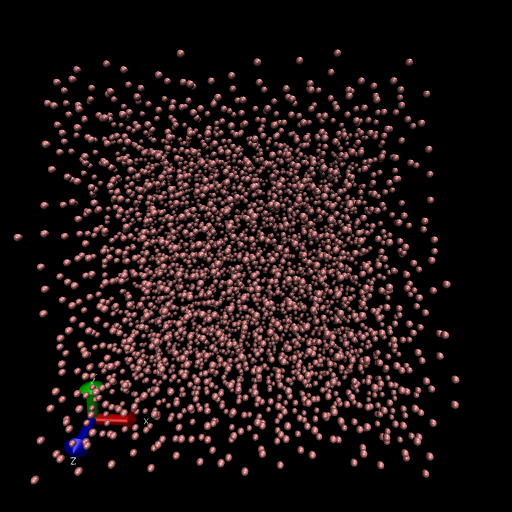
\includegraphics[width=0.5\textwidth]{vmd_image.png}
	\end{center}
\end{figure}
\section{Conclusions and Future Work}

In conclusion, we set out to design a molecular dynamics (MD) simulation package that performed time reversible integration on a system of Lennard-Jones particles in the constant temperature (NVT) ensemble.  We accomplished this in an object-oriented, extensible fashion on CPUs and successfully extended our code to work on GPUs as well.  We implemented numerous optimizations including neighbor/cell lists and parallelization involving OMP.  We profiled and benchmarked code along the way to continuously improve our code and algorithms during development.  In addition, our code is extensible to other pair potential functions beyond Lennard-Jones, exemplified by the pairUF potential we provided for the CPU code.  We additionally made no restrictions involving the integration method (which is related to what ensemble we choose to work in) as demonstrated by our inclusion of an NVE class integrator.  Our constant-temperature integration scheme is a time-reversible implementation of the Nos\'{e}-Hoover thermostat, which preserves the dynamics of these systems, hence our ability to obtain mean-squared displacement plots, etc.  Finally we compared our code against publicly available MD packages and found quantitative agreement.  We have thus accomplished all our goals, and a few more, we originally laid out for this project.



\pagebreak
\bibliographystyle{proteins1}
\bibliography{references}

\end{document}
